\documentclass[10pt,a4paper]{article}
\usepackage[utf8]{inputenc}
\usepackage[margin=17mm,top=20mm,bottom=18mm]{geometry}
\usepackage{fontenc}
\usepackage{xcolor}
\usepackage{tabularx,booktabs,array}
\usepackage{enumitem}
\usepackage{tcolorbox}
\usepackage{tikz}
\usetikzlibrary{arrows.meta,positioning}
\usepackage{hyperref}
\usepackage{fancyhdr}
\usepackage{titlesec}
\pdfmapfile{+cm.map}
\DeclareFontShape{TS1}{cmr}{m}{n}{<-> cmr10}{}

\definecolor{navy}{HTML}{12263A}
\definecolor{teal}{HTML}{087F7A}
\definecolor{mint}{HTML}{E9F7F3}
\definecolor{sky}{HTML}{EFF4FA}
\definecolor{ink}{HTML}{203346}
\definecolor{muted}{HTML}{657486}
\definecolor{edge}{HTML}{D7E3EA}
\definecolor{amber}{HTML}{B77816}
\definecolor{sand}{HTML}{FFF7E9}

\hypersetup{colorlinks=true,urlcolor=teal,linkcolor=teal,pdfauthor={Network Programming Group},pdftitle={ThogaMura - Group Proposal v2 - Java Network Programming}}
\setlength{\parindent}{0pt}
\setlength{\parskip}{3.5pt}
\setlist[itemize]{label=$\bullet$,leftmargin=*,itemsep=1.5pt,topsep=1.5pt}
\setlist[enumerate]{leftmargin=*,itemsep=1.5pt,topsep=1.5pt}
\renewcommand{\arraystretch}{1.22}
\titleformat{\section}{\Large\bfseries\color{navy}}{}{0pt}{}
\titleformat{\subsection}{\normalsize\bfseries\color{teal}}{}{0pt}{}
\titlespacing*{\section}{0pt}{6pt}{4pt}
\titlespacing*{\subsection}{0pt}{6pt}{2pt}
\pagestyle{fancy}
\setlength{\headheight}{20pt}
\fancyhf{}
\fancyhead[L]{\footnotesize\bfseries\color{teal} THOGAMURA}
\fancyhead[R]{\footnotesize\color{muted} NETWORK PROGRAMMING / ASSIGNMENT 02}
\fancyfoot[L]{\footnotesize\color{muted} Team review v2 \quad | \quad 17 November 2026}
\fancyfoot[R]{\footnotesize\color{muted} \thepage}
\renewcommand{\headrulewidth}{0.4pt}
\renewcommand{\headrule}{\hbox to\headwidth{\color{edge}\leaders\hrule height \headrulewidth\hfill}}

\newtcolorbox{infobox}[1][]{colback=mint,colframe=edge,boxrule=0.7pt,arc=2mm,left=3mm,right=3mm,top=2.5mm,bottom=2.5mm,#1}
\newtcolorbox{plainbox}[1][]{colback=sky,colframe=edge,boxrule=0.7pt,arc=2mm,left=3mm,right=3mm,top=2.5mm,bottom=2.5mm,#1}
\newtcolorbox{warnbox}[1][]{colback=sand,colframe=amber!45,boxrule=0.7pt,arc=2mm,left=3mm,right=3mm,top=2.5mm,bottom=2.5mm,#1}
\newcommand{\eyebrow}[1]{{\small\bfseries\color{teal}\MakeUppercase{#1}}}
\newcommand{\quiet}[1]{{\color{muted}#1}}
\newcommand{\tagline}[1]{{\small\bfseries\color{teal}#1}}
\newcommand{\member}[4]{%
  \begin{tcolorbox}[colback=white,colframe=edge,boxrule=0.7pt,arc=2mm,left=3mm,right=3mm,top=2.2mm,bottom=2.2mm]
    {\large\bfseries\color{navy}#1}\hfill{\small\bfseries\color{teal}#2}\par
    \textbf{Why useful:} #3\par
    \textbf{Deliver and demo:} #4
  \end{tcolorbox}%
}

\begin{document}

% PAGE 1 -- IDEA AND PURPOSE
\vspace*{5mm}
\eyebrow{Network Programming / Five-member group proposal}

{\Huge\bfseries\color{navy} ThogaMura}\par
\vspace{2mm}
{\Large\color{teal} Branch-to-warehouse stock coordination}\par
\vspace{4mm}
\begin{tcolorbox}[colback=navy,colframe=navy,arc=2mm,left=5mm,right=5mm,top=4mm,bottom=4mm]
{\large\bfseries\color{white} One clear idea}\par
{\color{white} Shop staff request inventory from a central warehouse. The system reserves stock safely, shows pick/dispatch progress, survives uncertain network replies, and lets staff check advisory supplier availability when warehouse stock is insufficient.}
\end{tcolorbox}

\section*{01 \quad The real-world problem}
Phone calls, paper notes and scattered chat messages make branch-to-warehouse coordination difficult. Two shops might request the last items at once; warehouse updates may be missed; a dropped network response can leave staff uncertain whether a request succeeded.

\begin{tabularx}{\linewidth}{>{\bfseries\color{ink}}p{0.24\linewidth} X X}
\toprule
Situation & Operational risk & ThogaMura response\\
\midrule
Competing requests & Stock is promised twice & One transactional reservation decision\\
Uncertain submission & A retry creates a duplicate & Command UUID and durable response replay\\
Dispatch visibility & Branches repeatedly call for status & Central NIO change hints plus fresh lookup\\
Warehouse stockout & Staff cannot quickly assess alternatives & Read-only supplier availability over HTTP\\
Untrusted endpoint & Commands reach an impostor server & Validated TLS server identity\\
\bottomrule
\end{tabularx}

\section*{02 \quad What we will build}
\begin{infobox}
\textbf{One connected Java networking application, five distinct implementations.} Next.js is only the browser interface, Spring Boot provides Java application lifecycle and HTTP bridging, and PostgreSQL stores authoritative inventory. The assessed networking code uses actual JDK \texttt{java.net}, \texttt{java.nio}, threading and JSSE APIs across processes.
\end{infobox}

\textbf{MVP scope:} products, one-SKU stock requests, reservation, ACCEPTED--PICKED--DISPATCHED status, movement history, change notification, safe retries, supplier inquiry and TLS command transport.

\textbf{Not MVP:} accounting, invoicing, payment, purchasing, automatic supplier orders, offline branch queue, AI, multiple warehouses and commercial supplier integration.

\begin{warnbox}
\textbf{Status: planning document, not a finished application.} The current GitHub repository contains a starter scaffold and tasks. Names are not assigned. Lecturer approval of the five lecture-concept allocations is still required, especially the HTTP/URL contribution for Member 2.
\end{warnbox}

\newpage

% PAGE 2 -- NETWORK ARCHITECTURE
\section*{03 \quad How it works over the network}
\begin{enumerate}
\item A branch operator opens the Next.js web UI on the \textbf{branch laptop}, which uses a local Spring Boot gateway.
\item The gateway sends a framed Java \textbf{TLS/TCP} command to the \textbf{central warehouse Java server} using a configured hostname/IP.
\item The server processes the command through bounded workers, checks PostgreSQL, and atomically accepts or rejects the reservation.
\item The server sends a minimal \textbf{Java NIO change signal} to connected branch gateways; the gateway triggers browser SSE and fetches authoritative state.
\item Warehouse staff pick and dispatch the request; on dispatch, the database records one movement and updates both on-hand and reserved quantities.
\item If warehouse stock is unavailable, an optional \textbf{Java HTTP/URL} connector queries a separately running supplier service for advisory availability.
\end{enumerate}

\section*{04 \quad Two-machine demonstration topology}
\begin{center}
\begin{tikzpicture}[font=\small, >={Latex[length=2.2mm]},
  base/.style={rounded corners=2mm,draw=edge,thick,align=center,minimum height=14mm,inner sep=3mm},
  branch/.style={base,fill=navy,text=white,minimum width=63mm},
  central/.style={base,fill=mint,minimum width=63mm},
  aux/.style={base,fill=sky,minimum width=55mm},
  conn/.style={->,thick,color=teal}
]
\node[branch] (client) at (0,0) {Branch laptop\\Next.js + Spring gateway};
\node[central] (server) at (9,0) {Warehouse laptop\\Java network server};
\node[aux,below=18mm of client] (supplier) {Independent supplier HTTP mock\\(read-only demo)};
\node[aux,below=18mm of server] (db) {PostgreSQL\\authoritative stock};
\draw[conn] ([yshift=3mm]client.east) -- node[above,font=\footnotesize] {TLS/TCP commands (M1+M5)} ([yshift=3mm]server.west);
\draw[conn] ([yshift=-3mm]server.west) -- node[below,font=\footnotesize] {NIO change hints (M3)} ([yshift=-3mm]client.east);
\draw[conn] (server.south) -- (db.north);
\draw[conn] (server.south west) to[bend left=12] node[below,font=\footnotesize,sloped] {HTTP availability (M2)} (supplier.north east);
\end{tikzpicture}
\end{center}

\begin{plainbox}
\textbf{Why this architecture is defensible:} The branch gateway and the central warehouse actually run on different machines for demonstration. TCP handles reliable command exchange and replay; NIO handles lightweight multi-gateway invalidation. They are independent responsibilities, not two names for the same feature.
\end{plainbox}

\section*{05 \quad Inventory correctness example}
If physical \textbf{on-hand = 10}, an accepted request for 8 changes \textbf{reserved = 8}, leaving \textbf{available = 2}. Picking does not subtract stock. Dispatch makes \textbf{on-hand = 2} and \textbf{reserved = 0}, and stores exactly one movement. Another simultaneous request for 8 cannot also succeed.

\begin{warnbox}
\textbf{Honest deployment boundary:} UDP discovery was removed because a configured server address is sufficient. The NIO feed in this course MVP is version-only and restricted to a private, firewall-controlled demo LAN; it is \textbf{not safe to expose on the public internet}. Production use requires HTTPS/user authorization and encrypted/authenticated notification transport or a secure VPN.
\end{warnbox}

\newpage

% PAGE 3 -- MEMBERS 1 TO 3
\section*{06 \quad Individual networking workloads: M1--M3}
\quiet{Indicative effort includes implementation, focused tests and one live negative-case demo; estimates are not deadlines.}

\member{Member 1 -- Reliable stock commands}{TCP / 12--16 hours}
{A branch and the central warehouse must exchange request/response messages, even when connections split data or drop after a database commit.}
{Build Java \texttt{Socket}/\texttt{ServerSocket} framed messages, request UUID correlation, timeouts, retry with the \emph{same} UUID and proper cleanup. Demonstrate split/merged TCP frames and a lost response that does \emph{not} create a second reservation. Integrate with M4's durable receipts and M5's TLS socket factory.}

\vspace{2mm}
\member{Member 2 -- Supplier availability inquiry}{HTTP/URL / 12--16 hours}
{When the warehouse cannot supply an SKU, staff can request an advisory quantity from another system without altering warehouse stock.}
{Implement Java \texttt{URI}, \texttt{URL} and \texttt{HttpURLConnection} client plus an \emph{independent} supplier HTTP mock process. Show a real 200 response, a known zero, 404 unknown, 503 outage, timeout and invalid JSON. No arbitrary URLs, fake availability or automatic purchase. The mock is not a live commercial supplier API.}

\vspace{2mm}
\member{Member 3 -- Multi-gateway status updates}{Java NIO / 16--22 hours}
{Several shop gateways need quick warehouse change hints without every browser polling continuously.}
{Build a Java \texttt{Selector}/\texttt{ServerSocketChannel}/\texttt{SocketChannel} notification feed with \texttt{ByteBuffer}, partial-write handling, bounded per-client queues and reconnect. Show ten gateway-like clients, a slow subscriber and post-disconnect authoritative refetch through Spring SSE. The feed is best effort, not durable truth.}

\section*{Ownership rule}
Every student must be able to identify their own classes, JDK APIs, input/output messages, automated tests and failure demonstration. Shared Next.js pages do \textbf{not} replace a member's networking feature.

\newpage

% PAGE 4 -- MEMBERS 4 TO 5 + SHARED
\section*{07 \quad Individual networking workloads: M4--M5}

\member{Member 4 -- Safe concurrent reservation}{Threads + DB / 16--22 hours}
{Simultaneous branch requests cannot promise more units than exist, and retries cannot apply a business action twice.}
{Use a bounded \texttt{ExecutorService} for request processing and PostgreSQL transactions with row locks or conditional updates for reservation, command receipt replay, PICKED/DISPATCHED transitions and movement uniqueness. Demonstrate two concurrent 8-of-10 requests, restart replay and double-dispatch protection. Java \texttt{synchronized} alone is not sufficient for database correctness.}

\vspace{3mm}
\member{Member 5 -- Secure socket transport}{JSSE/TLS / 12--16 hours}
{The branch must verify that it is speaking to the trusted warehouse server and protect command data in transit.}
{Implement validated \texttt{SSLSocket}/\texttt{SSLServerSocket} setup, per-developer certificates/truststores outside Git, hostname verification and fail-closed behavior. Demonstrate a trusted command and refusal of an untrusted or wrong-name certificate; no plaintext fallback. TLS does not itself authorize individual staff accounts.}

\section*{08 \quad Shared work: divide fairly}
\begin{tabularx}{\linewidth}{>{\bfseries\color{ink}}p{0.29\linewidth} X}
\toprule
Work package & Shared responsibilities\\
\midrule
Next.js frontend & Products, requests, warehouse queue, advisory supplier view, accessible errors and reconnect warnings\\
Spring gateway wiring & REST/SSE mapping, user-visible statuses, configured warehouse host and proper error handling\\
Integration and review & Freeze contracts, two-machine LAN tests, interface reviews, secure NIO demo restrictions\\
Report and submission & Diagram, screenshots, personal code evidence, PDF report and single Moodle ZIP\\
\bottomrule
\end{tabularx}

\begin{infobox}
\textbf{Fairness approach:} M3 and M4 have the highest technical risk and should receive extra peer testing support. M2 owns its mock service as well as the actual HTTP connector and failure UI evidence so its assignment is not merely one HTTP call. Final effort is reviewed after the team knows everyone's strengths.
\end{infobox}

\section*{09 \quad What each member must show}
\begin{itemize}
\item \textbf{Working network boundary:} two separate processes, not a direct Java method call.
\item \textbf{Happy path + failure path:} observed outputs, resource cleanup and test evidence.
\item \textbf{Unique lecture concept:} explain the relevant JDK types and why that networking design serves the actual workflow.
\end{itemize}

\newpage

% PAGE 5 -- ROADMAP AND SIGN-OFF
\section*{10 \quad Suggested five-week plan}
\begin{tabularx}{\linewidth}{>{\bfseries\color{teal}}p{0.16\linewidth} X >{\raggedright\arraybackslash}p{0.30\linewidth}}
\toprule
Stage & Primary deliverables & Demonstrable gate\\
\midrule
Week 1 & Agree protocol/contract, freeze five assignments, two-JVM TCP PING, PostgreSQL setup, supplier mock skeleton & Real socket call between processes\\
Week 2 & TCP/TLS command path, durable reservation, request frontend, idempotent replay & Browser request creates one DB decision\\
Week 3 & NIO multi-gateway hints, supplier HTTP connector, warehouse pick/dispatch & Five visible network flows\\
Week 4 & Timeout/slow-reader/race/cert negative tests, private-NIO restrictions, UI states & Each member success + failure demo\\
Week 5 & Two-machine rehearsal, report evidence, full source ZIP and one Moodle submission & Clean-clone verification and group demo\\
\bottomrule
\end{tabularx}

\section*{11 \quad Five-minute group explanation}
\begin{plainbox}
\textbf{ThogaMura is a stock coordination system between branch shops and a central warehouse.} Shops can request inventory; the server reserves it without double allocation, warehouse staff dispatch it, and branches see updates. If stock is unavailable, staff can ask a supplier service for advisory availability. Five members each implement a different networking concept: TCP requests, HTTP/URL supplier inquiry, NIO live signals, multithreaded reservation, and TLS security.
\end{plainbox}

\section*{12 \quad Decisions before implementation}
\begin{enumerate}
\item Confirm the five distinct lecture concepts with the lecturer, especially Member 2's Java HTTP/URL programming.
\item Confirm group member names/GitHub handles and assign the currently \textbf{unassigned} issues by M1--M5 prefix.
\item Freeze the command and supplier HTTP contracts; confirm which laptops will host gateway, warehouse and supplier mock.
\item Agree that public internet operation, real supplier integration, staff authentication and offline queues are \textbf{outside this coursework MVP}.
\end{enumerate}

\section*{13 \quad Submission and links}
The assignment requires one group ZIP with complete source code \textbf{and a final implementation report PDF}. This document is the \textbf{idea proposal}, not that final report. The final report must contain real member contributions, testing, screenshots and observed results.

\textbf{Repository:} \href{https://github.com/Suthankan1/ThogaMura}{github.com/Suthankan1/ThogaMura}\\
\textbf{Workload details:} \href{https://github.com/Suthankan1/ThogaMura/blob/main/docs/TEAM_WORKLOADS.md}{docs/TEAM\_WORKLOADS.md}\\
\textbf{Issue index:} \href{https://github.com/Suthankan1/ThogaMura/issues/1}{GitHub issue \#1}\\
\textbf{Design source:} \href{https://github.com/Suthankan1/ThogaMura/blob/main/docs/NETWORK_FEATURES_V2.md}{docs/NETWORK\_FEATURES\_V2.md}

\vfill
{\footnotesize\color{muted}Technical references: Java SE 21 \texttt{java.net}, \texttt{java.nio.channels} and JSSE; PostgreSQL transaction and locking documentation; group-provided lecture PDFs; Assignment 02 instructions.}\par

\end{document}
